\chapter{Introduction}
In the Field of combinatorial optimization, the Traveling Salesman Problem (TSP) stands out as a timeless and extensively researched challenge. Despite its deceptively simple formulation, finding a solution proves to be an extremely intricate task, earning it a reputation as one of the most notorious NP-complete problems \cite{np_comp}. The significance of TSP lies in its far-reaching practical implications, influencing fields such as logistics, transportation planning, robotics, and manufacturing, where efficient distribution and task sequencing are crucial. By cracking the TSP code, substantial gains can be made in terms of time, resources, and financial savings.

\noindent The purpose of this paper is to present, analyze and compare different approaches to solve the Traveling Salesman Problem \cite{10.5555/1614191} as a way to understand more deeply the various issues that arise when approaching those kind of problems.

\section{Formulation of this thesis}
In the next chapters, we are going to present all the work done, which includes mathematical formulations, implementation, and testing phases. In particular, this report is structured as follows:

\begin{description}
    \item[Chapter 1:] TSP History and formulation, providing a comprehensive overview of the Traveling Salesman Problem.
    \item[Chapter 2:] Heuristics, detailing two heuristics approaches used to find approximate solutions to the TSP and discussing their efficiency and applicability.
    \item[Chapter 3:] Metaheuristics, exploring advanced metaheuristic techniques and their effectiveness when applied to the TSP.
    \item[Chapter 4:] Exact Models, presenting exact solution methods with a focus on their implementation and performance.
    \item[Chapter 5:] Matheuristics, combining mathematical programming and heuristic methods to create hybrid approaches, and evaluating their performance on TSP instances.
    \item[Chapter 6:] Conclusions, summarizing the findings, discussing the strengths and limitations of the different methods.
\end{description}

\noindent The code, this thesis, and further information can be found in the following GitHub repository: \url{https://github.com/Piero24/TSP_Optimization}


\section{Problem history}
The Traveling Salesman Problem (TSP) is a Combinatorial Optimization problem, succinctly posed as follows: "What is the shortest route a traveling salesman can take to visit \( n \) cities and return back to his home city, only traversing each city once?" \\

\noindent The origins of the Traveling Salesman Problem (TSP) are shrouded in uncertainty, making it difficult to pinpoint its exact roots. However, one plausible theory dates the problem back to 1856-57 with William Hamilton. Hamilton created the "Icosian Game," which involved finding a path along the edges of a dodecahedron that visits every vertex exactly once, traverses no edge twice, and returns to the starting point. This concept, now recognized as a Hamiltonian Circuit, laid the groundwork for the Traveling Salesman Problem \cite{biron2006}. \\

\noindent An alternative hypothesis suggests that the problem may have been formulated even earlier, potentially originating from a 1832 German handbook titled "\textit{The traveling salesman – how he should be and what he should do, to get the orders and assure success for his business – from an old traveling salesman.}"

The book features five routes that traverse regions of Germany and Switzerland. Notably, four of these routes involve revisiting an earlier city, which serves as a base for that leg of the journey. In contrast, the fifth route stands out as a genuine traveling salesman tour, as characterized in Alexander Schrijver's comprehensive book on combinatorial optimization \cite{unknown:TSP}. An illustration of the tour is given in Figure \ref{fig:TSP_path}. 

\begin{figure}
    \centering
    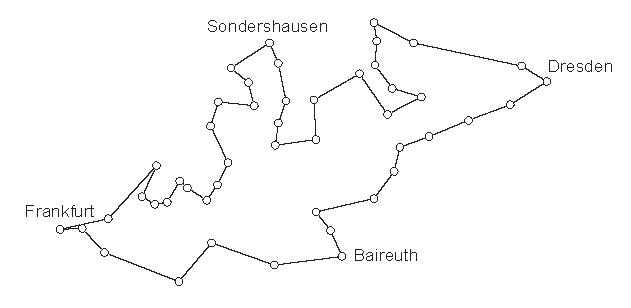
\includegraphics[width=0.9\linewidth]{Immagini/TsP_path.pdf}
    \caption{The Commis-Voyageur tour.}
    \label{fig:TSP_path}
\end{figure}

\noindent The first mathematical papers on the Traveling Salesman Problem (TSP) date back to 1940. Initially, researchers focused on finding a lower bound for the optimal tour. This interest was sparked by a practical problem encountered during an expedition in Bengal, where the transportation of men and materials between locations was a major expense.\\

\newpage

\noindent Mathematicians subsequently generalized the problem, first considering a finite number of random points within a unit-sided square, and later expanding to a general area. During this period, Ghosh observed that the problem proved to be extremely complex, except for very small instances, which, although solvable, held little practical significance. \\

\noindent The term "Traveling Salesman Problem" (TSP) was first mentioned in a 1949 report by Julia Robinson, but it is likely that the name was already in use at Princeton in the 1930s or 1940s. In the 1940s, mathematicians at RAND Corporation, including Merrill Flood, began studying the problem in earnest. In 1954, a team of researchers at RAND, including Dantzig, Fulkerson, and Johnson, made a significant breakthrough by solving a 49-city problem in the USA using the simplex method.

Since then, improvements in solving the TSP have come mainly from developing better methods for applying the cutting plane method to linear programming problems. While there have been no major theoretical breakthroughs, researchers have made progress in understanding the TSP polytope and its properties, as well as developing heuristic algorithms to find near-optimal solutions. A notable theoretical result is the proof of the NP-hardness of the decision version of the TSP in 1972.

In the 1990s, Applegate, Bixby, Chvátal, and Cook developed the program Concorde that has been used in many recent record solutions. Gerhard Reinelt published the TSPLIB in 1991 \cite{TSPLIB95}, a collection of benchmark instances of varying difficulty, which has been used by many research groups for comparing results. In 2006, a team of researchers computed an optimal tour for an 85,900-city instance, currently the largest solved instance. For many other large instances, solutions can be found that are within 2-3\% of an optimal tour \cite{wiki:TSP}.

Today, the research on the TSP is very active and its results have been successfully applied to other Operations Research problems. On one side, there is the search for better heuristics, both for speed and for optimality, using for example simulated annealing, genetic algorithms, tabu-search, neural networks or ant-colonies. On the other side, researchers have developed better and better software to solve the TSP to optimality, mainly through variants of the cutting plane method \cite{fortini2007lp}.


\section{Problem formulation}
The Traveling Salesman Problem (TSP) consists in finding a Hamiltonian circuit of minimum cost on a given directed graph \( G = (V, E) \). In some cases, the problem can be analogously defined on a undirected graph; this happens when the cost associated with an arc does not depend on its orientation \cite{fischetti2019}. In the context of directed graphs, the goal is to find a path that traverses each arc exactly once while minimizing the total cost. Similarly, in undirected graphs, the problem is equivalent when the cost of traversing an edge is symmetric and independent of its direction. \\

\noindent In this document, we primarily address the Symmetric Traveling Salesman Problem (STSP), a fundamental challenge in combinatorial optimization. In STSP, we deal with an undirected weighted complete graph \( G = (V, E) \), where \( V = \{v_1, \ldots, v_n\} \) represents a set of \( n \) nodes, and \( E \) comprises the set of \( n \) edges. Each edge \( e = \{i, j\} \in E \) is associated with a non-negative real number, represented by the function \( c: E \rightarrow \mathbb{R}^+ \), denoting arbitrary distances or weights between nodes. \\

\noindent As mentioned before, the fundamental goal of the Traveling Salesman Problem (TSP) is to identify the most efficient sequence of edges or nodes that form a tour with the minimum total cost, also known as an optimal tour. To address this task, we need to formulate the problem as an integer linear program. Two notable formulations are the Miller--Tucker--Zemlin (MTZ) formulation and the Dantzig--Fulkerson--Johnson (DFJ) formulation. While the DFJ formulation is stronger, the MTZ formulation remains useful in specific contexts \cite{wiki:TSP}.

\newpage

\subsection{Dantzig–Fulkerson–Johnson (DFJ)}
\label{chap:DFJ}
In this paper, we consider the Dantzig–Fulkerson–Johnson formulation. It is constructed as follows: each city is identified by a unique label from \(1, \ldots, n\), and the cost (or distance) of traveling from city \(i\) to city \(j\) is represented by the positive value \(c_{e} > 0\). The central variables in this model are \(\{x_{e}\}_{i,j}\), where \(x_{e}\) represents the decision variable associated with traveling from city \(i\) to city \(j\). They are constructed as follows:

\begin{align}
    x_{e} = 
    \begin{cases}
        1 & \text{the path goes from city $i$ to city $j$} \\
        0 & \text{otherwise}
    \end{cases}
\end{align}

The presence of $0/1$ variables in this formulation transforms them into integer programs, while all other constraints remain linear. Specifically, the objective of the program is to minimize the total tour length, which is represented by:

\begin{align}
    \quad \sum_{e \in E} c_e x_e.
\end{align}

Without additional constraints, the variables $\{x_{ij}\}_{i,j}$ would essentially span all possible subsets of edges, which is far from the edges that form a tour. This would allow for a trivial minimum solution where all $x_{ij} = 0$. To avoid this, the formulation include the constraints that each vertex has exactly one incoming edge and one outgoing edge, which can be represented by $2n$ linear equations.
The optimization problem is defined as follows:

\begin{align}
    \text{min} \quad & \sum_{e \in E} c_e x_e \label{eq:eq1}\\ 
    \quad & \sum_{e \in \delta(v)} x_{e} = 2 \quad \forall v \in V \label{eq:eq2}\\
    & \sum_{e \in E(Q)} x_{e} \leq |Q| - 1 \quad \forall \ Q \subset V:|Q| \geq 2 \label{eq:eq3}\\
    & 0 \leq x_e \leq 1 \text{ integer} \quad \forall e \in E \label{eq:eq4}
\end{align}

\noindent Constraints \ref{eq:eq2} ensure that each node in the graph is visited by exactly two edges of the cycle. 

\newpage

\noindent However, these constraints alone are not sufficient to guarantee a valid Hamiltonian Cycle, as the solution may consist of multiple isolated cycles. The final constraint in the DFJ formulation \ref{eq:eq3}, also known as a Subtour Elimination Constraint (SEC), ensures that any solution found using this model consists of a single connected component. Specifically, this constraint prevents any proper subset \( Q \) from forming a sub-tour, ensuring that the solution is a single tour rather than a collection of smaller tours. Due to the exponential number of possible constraints, the problem can be very difficult to solve so this is typically solved using row generation in practice \cite{wiki:TSP}.